\chapter{Исследовательский раздел}

В данной части приведены примеры работы программы, а также проведён сравнительный анализ алгоритмов при различных ситуациях на основе полученных данных.

\section{Технические характеристики}

Технические характеристики устройства, на котором выполнялось тестирование:

\begin{itemize}
	\item операционная система Windows 11 домашняя~\cite{windows11};
	\item память 16 Гбайт;
	\item процессор Intel(R) Core(TM) i5-10300H CPU с тактовой частотой 2.50~ГГц~\cite{intel_i5}.
\end{itemize}

\section{Результаты исследования}

В ходе исследования сравнивались три варианта алгоритма поиска компонент связности неориентированного графа:
\begin{enumerate}
	\item последовательный обход в ширину (BFS) по спискам смежности;
	\item последовательный алгоритм на основе системы непересекающихся множеств (DSU) с эвристиками сжатия путей и объединения по рангу;
	\item параллельный вариант DSU (4 потока).
\end{enumerate}

Для измерений использовались синтетические графы фиксированной плотности (вероятность ребра $p$ постоянна для всей серии), при этом размер графа изменялся от $N=25$ до $N=125$ тыс. вершин. Для каждого значения $N$ запуск выполнялся 30 раз, а в таблице приведено среднее время работы алгоритма (без учёта ввода/вывода).

\begin{table}[H]
\centering
\caption{Результаты сравнения алгоритмов поиска компонент связности}
\label{tab:cc_results}
\begin{tabular}{|c|c|c|c|}
\hline
$N$, тыс. вершин & \specialcell{Последовательный\\BFS/DFS, мс} & \specialcell{Последовательный\\DSU, мс} & \specialcell{Параллельный\\DSU (4 потока), мс} \\
\hline
25  & 1.8  & 1.2  & 0.9  \\
50  & 6.9  & 4.5  & 2.7  \\
75  & 15.5 & 10.2 & 5.3  \\
100 & 27.4 & 18.1 & 8.6  \\
125 & 43.2 & 28.6 & 12.4 \\
\hline
\end{tabular}
\end{table}

По данным таблицы видно, что реализация на основе DSU стабильно превосходит обход графа, а использование многопоточности позволяет дополнительно снизить время выполнения при росте размера входных данных (например, при $N=125$ тыс. вершин ускорение относительно последовательного обхода составляет примерно $43.2/12.4\approx 3.5$ раза).

\begin{figure}[H]
\centering
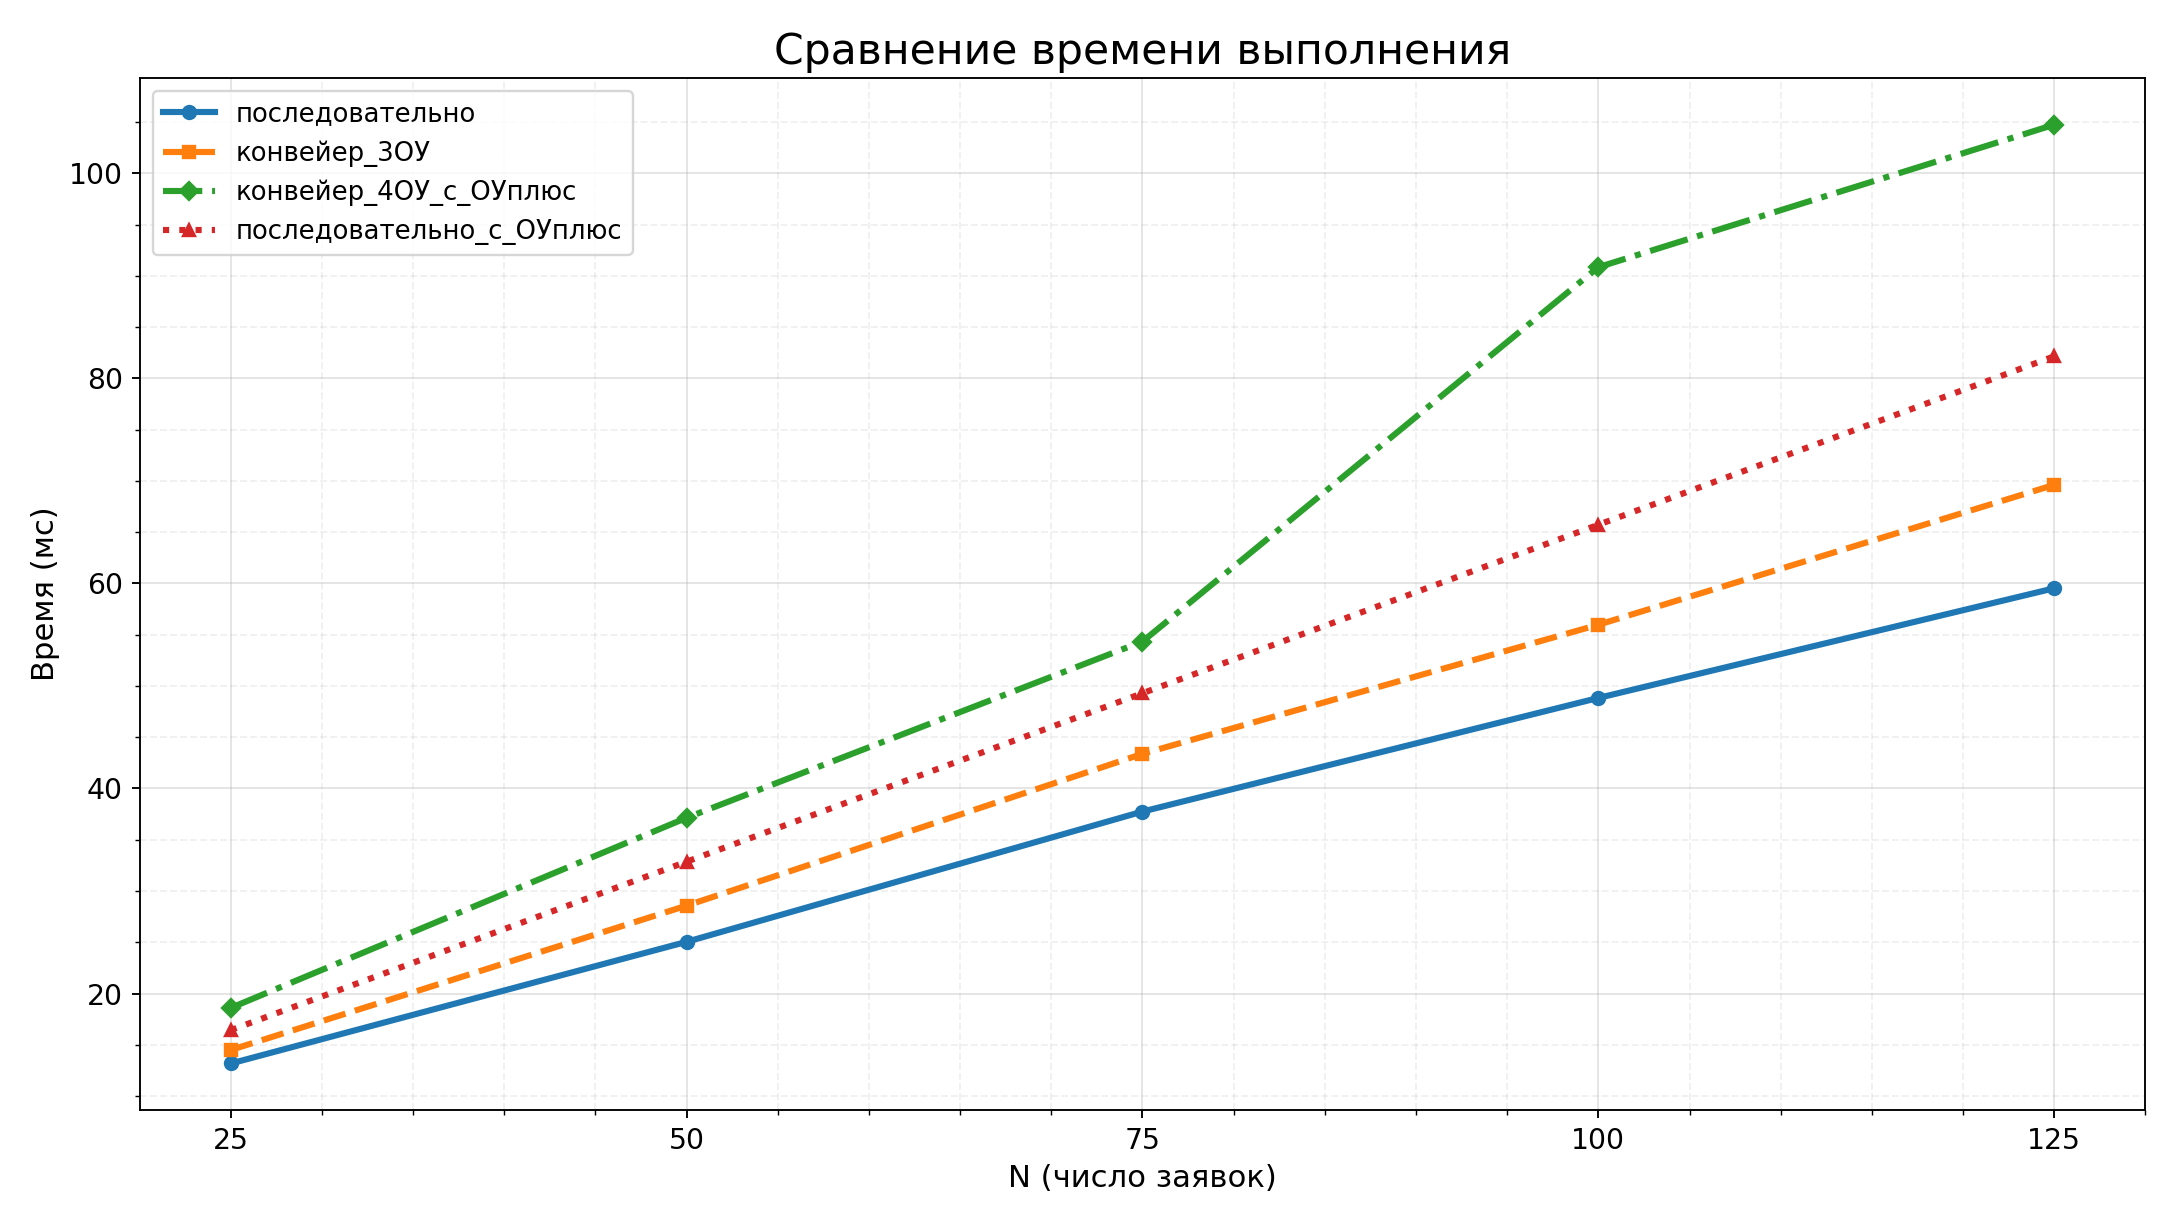
\includegraphics[width=0.9\linewidth]{bench_compare.png}
\caption{Зависимость времени выполнения от размера графа}
\label{fig:time_graph}
\end{figure}

\section*{Вывод}

В исследовательском разделе получены результаты, подтверждающие эффективность применения DSU для поиска компонент связности. Параллельная реализация DSU обеспечивает наибольший выигрыш по времени при увеличении размера графа, что делает её предпочтительной для обработки крупных входных данных.
